
\documentclass[runningheads]{llncs}

\usepackage{amssymb}
\usepackage[english]{babel}
\usepackage[utf8]{inputenc}
\setcounter{tocdepth}{3}
\usepackage{graphicx}

\usepackage{url}
\urldef{\mailsa}\path|{jrra,ksma,atka}@itu.dk|
\newcommand{\keywords}[1]{\par\addvspace\baselineskip
\noindent\keywordname\enspace\ignorespaces#1}
\graphicspath{{images/}}

\begin{document}

\mainmatter  % start of an individual contribution

% first the title is needed
\title{Model-Driven Development Project:\\ Modelling, Domain-Specific Language\\ and Code Generation}

% a short form should be given in case it is too long for the running head
\titlerunning{Model-Driven Development Project}

\author{Jacob Romme Rasmussen \and \\ Kristian Støving Mørk Andersen \and \\ Athanasios Kastanidis}
%
\authorrunning{Model-Driven Development Project}

\institute{\mailsa\\}

\toctitle{Lecture Notes in Computer Science}
\tocauthor{Authors' Instructions}
\maketitle


\begin{abstract}
This paper covers the process of modelling and structuring an external domain-specific language with the sole purpose of writing surveys. The language comes with its own editor and compiler. Code is automatically generated from the constructed surveys and targets multiple platforms, namely the Android mobile platform and a web platform. 
\keywords{Model-driven development, Meta-model, DSL, Code generation, Android, HTML}
\end{abstract}

\section{Introduction}

This paper describes the design and implementation of a Domain Specific Language (DSL) for generating survey applications. The purpose of the project is to design a language that can be used by a non-programmer to define surveys. These surveys can then be used to generate applications for answering surveys on multiple platforms. This reduces the amount of code duplication a programmer would generally encounter while writing a survey application for multiple platforms. In turn this also reduces the time development takes. Most importantly the survey DSL along with the code generation tool can be used to generate and endless number of survey applications without rewriting any code.

\section{System Overview}
This section seeks to provide an overview of the system as a whole. The system is visualized as a model hierarchy in figure \ref{fig:mhier} and is an adaptation of the Object Management Group\cite{omg} modeling architecture. Additional system details have been added to provide more information about the system flow - that is, where and when various programming-specific tasks take place.
\begin{figure}
\centering
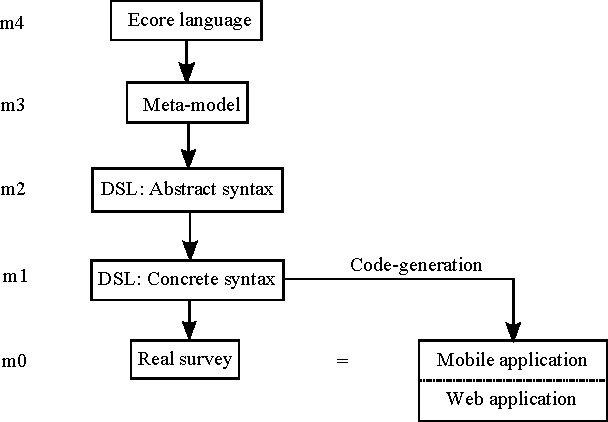
\includegraphics[height=6.2cm]{modelhierarchy}
\caption{A figure depicting the model hierarchy of the system. The m-levels are a notation adopted by the Object Management Group\cite{omg} modeling architecture.}
\label{fig:mhier}
\end{figure}
The Ecore language is placed at the top level of the system which makes it possible to construct a meta-model of our language. Together with the abstract syntax, the structure and relations of the meta-model is passed to the concrete syntax at level m1. At this level, a language-specific file (*.survey) is the center of attention. Constraints are checked against this file and code is generated from this file. The real survey is placed on the bottom level and can take on different forms. In our case, we are concerned with files that provide the core of an Android application and a web application.

\section{Language Design}
%Domain analysis and the meta-model
%Concrete-syntax (interesting aspects of the grammar)
%How and what design principles you followed? (cite literature) \\
When performing the domain analysis we searched for the most popular online survey sites and chose to use the survey templates provided by Surveymonkey\cite{surveymonkey} and Obsurvey\cite{obsurvey} as inspiration. The language is specifically designed to support their survey design. The surveys span a variety of different types of questions. Multiple answers can be given to some questions, while others only allow a single answer. Most answers are preset, while some allows the user to type free text. A question can contain answers of both types. The questions are either listed on a single page or divided into several pages. A question can depend on previous answers meaning it is only shown if a certain answer was chosen earlier. This is useful when some answers make the following questions irrelevant. The combined functionality of the investigated surveys lead to the following requirements for the survey system:
\begin{itemize}
\item  A survey must contain at least one question. 
\item A question has a type indicating the amount and types of answers allowed. 
\item A question can require specific previous answers and should only be made available if all the required answers were chosen by the user. 
\item Multiple choice questions allow users to choose multiple predefined answers.
\item RadioChoice questions should only allow a single answer. 
\item Open questions do not contain any predefined answers but allow a user to define the answer themselves. 
\item An open question must contain a single open(not predefined) answer.
\end{itemize}
The structure of the meta-model shown in figure \ref{fig:mmod} is based on requirements listed previously and as such attempts to capture the structure of the investigated surveys. 
\begin{figure}
\centering
% 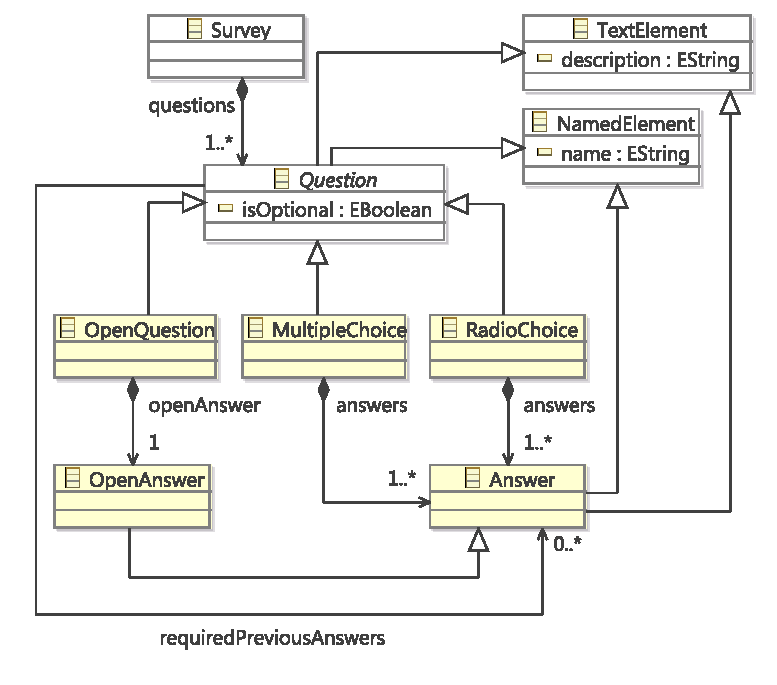
\includegraphics[height=6.2cm]{metamodel}
\caption{A figure depicting the metamodel of the DSL.}
\label{fig:mmod}
\end{figure}
The Survey root element contains one or more questions. The question entity is split into three subentities denoting the type of question. An alternative approach would be to merge the MultipleChoice and RadioChoice entities and use an enumeration to describe a question type attribute. However, we argue that it is visually more pleasing to have the distinct separation displayed in the model. A question contains one or more references to answers denoting the relevancy of the question. A constraint is run on the model checking that no question requires one of its own answers. The model provides the basis for the abstract syntax of the domain-specific language, which is used to write a survey in concrete syntax. During the design phase of the language we chose to follow a set of guidelines by Karsai, G., et al.\cite{karsai}. The main guidelines being 
\begin{quotation}
\emph{Keep it simple.} [...] \emph{Avoid unnecessary generality.}
\end{quotation}
This is reflected in the model which contains a minimum number of entities, and the concrete syntax which only contains the neccessary components to satisfy the requirements.
\medskip

\noindent
{\it Example of the concrete syntax in a *.survey-file is shown below}
\begin{verbatim}
multiple:
	"What is your favourite pet?"
	answer dogAnswer "Dogs"
	text otherAnswer "Something else?"

single:
	"Which is better - Coffee or tea?"
	optional
	requires dogAnswer
	answer teaAnswer "Tea"
	answer coffeeAnswer "Coffee" 

open:
	"Describe how you feel about Windows XP."
	optional
	text xpAnswer
\end{verbatim}
%
\noindent
A *.survey file contains one or more question-segments. A segment defines the type of the question followed by a surveyor-defined description - the actual question to be read by the surveyee. The optional-keyword is used to indicate if the question in the given segment is optional. The remainder of the segment contains a list of answers starting with the answer-keyword, followed by an identifier and a description (the actual predefined answer). The identifier is only used internally when referencing the answer from somewhere else in the file. The referencing of answers is used when \emph{requiring} that certain answers have been chosen by the surveyee in order for the question to be relevant. The naming of the keywords are chosen specifically to capture the essence of their functionality and be easily understandable by anyone with no prior programming experience or the like. When designing the concrete syntax of a domain-specific language, Karsai, G., et al.\cite{karsai} recommends that one should
\begin{quotation}
 \emph{Adopt existing notations domain experts use.}
\end{quotation}
Thus, many of the keywords are names of concepts used in the survey domain. The colon is commonly known to explain or define the preceeding element - here it is used to indicate the start of the definition and contents of a question. The main intention with the concrete syntax design is that only minor knowledge about surveys is enough to be able to use the DSL with ease. 

\section{Architecture of the language implementation}

We have chosen to model our language as an external DSL such that it can be independent of any other language. Our DSL does not require any functionality such as expression evaluation that may easily be handed down in an internal DSL. Therefore we have chosen to implement it as an external DSL. 

The first part of our system is an Android app which can be used to answer surveys. Because Android runs Java it would be easy to choose to run the DSL as interpreted language in the Android app. This would on the other hand make the app slower on the computationally constrained hardware Android runs within. Instead we have chosen to generate native Java code for the Android app to make it fast and easily adaptable to other platforms.\\

INSERT TEXT ABOUT THE WEB APP HERE!\\

The survey DSL itself is implemented using Xtext, an Open Source framework for development of programming languages and DSL's. Xtext is highly integrated with the code editor environment Eclipse. When developing a language using Xtext it is possible to generate Eclipse plugins automatically syntax highlight, lint and build files written. By using Xtext for our DSL we gain these capabilities with only little effort. 
% External DSL. Generating code. Model to text transformations
% Use of editor tools through Eclipse.
% Xtext and xtend.

% Testing

% Internal\/External DSL? Interpreted? Generating code? Use of
% model-to-model transformations?
% Reuse between different back-ends? Coupling between back-ends and
% between the front-end and the back-ends?
% Toolchain elements? What tools do you provide? What tools one could
% provide as an extension?
% Cogen argument about advantages of your architecture, maintainability,
% development cost.
% Are the requirements met?
% How did you test the implementation?

\begin{thebibliography}{4}

\bibitem{karsai} Karsai, G., Krahn, H., Pinkernell, C.,, Rumpe, B., Schindler, M., Völkel, S.: Design guidelines for domain specific languages. 
9th OOPSLA Workshop on Domain-Specific Modeling (2009), \url{http://www.dsmforum.org/events/dsm09/Papers/Karsai.pdf}

\bibitem{surveymonkey}SurveyMonkey, \url{http://www.surveymonkey.com/s/Public-School-Survey-Template}

\bibitem{obsurvey}Obsurvey, \url{http://www.obsurvey.com/language-proficiency-template/}

\end{thebibliography}

\end{document}
